\documentclass[a4paper,12pt]{refrep}
\usepackage[utf8]{luainputenc}
\usepackage{xcolor}
\usepackage{booktabs}
\usepackage{longtable}
\usepackage{tabularx}
\usepackage{rotating}
\usepackage{multicol}
\usepackage{multirow}
\usepackage[disable]{todonotes}
\usepackage{tocloft}
\usepackage{hyperref}
\usepackage{gensymb}
\makeatletter

% Font selection
\renewcommand{\familydefault}{\sfdefault}
\fontfamily{phv}\selectfont

% Reference colors
\hypersetup{
  unicode=true,
  linkcolor=blue, % internal links
  linktocpage=true, % only page numbers
  urlcolor=blue, % external links
  citecolor=green,
  filecolor=magenta,
  bookmarks=true,
  bookmarksnumbered=true,
  breaklinks=true, % wrap links is Ok
  colorlinks=true,
  pdftoolbar=true,
  pdfmenubar=true,
  pdfnewwindow=true
}

% Some shortcuts
\newcommand\xc{\textsf{XCSoar}}
\newcommand\fl{\textsf{Flarm}}
\newcommand\al{\textsf{Altair}}

% Define command to insert XCSoar website
\newcommand{\xcsoarwebsite}[1]{\url{https://xcsoar.org#1}}
\newcommand{\xcsoarforum}[1]{\url{https://forum.xcsoar.org#1}}

% Define command to insert tip image
\newcommand{\tip}[0]{\marginlabel{\parbox{1.1cm}{\includegraphics[width=0.7cm]{figures/reminder.pdf}}}}

% Define command to insert gesture image
\newcommand{\gesture}[1]{\marginlabel{{\it#1
}\parbox{1.3cm}{\includegraphics[width=0.7cm]{figures/gesture.pdf}}}}

% Define command to insert specific gesture image
\newcommand{\gesturespec}[1]{\marginlabel{\parbox{1.3cm}{\includegraphics[width=0.9cm]{figures/#1.png}}}}

% Define command to insert warning image
\newcommand{\warning}[0]{\marginlabel{\parbox{1.3cm}{\includegraphics[width=0.9cm]{figures/warning.pdf}}}}

% Define command to insert Achtung image
\newcommand{\achtung}[0]{\marginlabel{\parbox{1.3cm}{\includegraphics[width=2.5em]{figures/warning.pdf}}}}

% Define command to insert a flash image
\newcommand{\blitz}[0]{\marginlabel{\parbox{1.3cm}{\includegraphics[height=2.0em]{figures/reminder.pdf}}}}

% Define command to insert a stop
\newcommand{\halt}[0]{\marginlabel{\parbox{1.3cm}{\includegraphics[height=2.0em]{figures/warning.pdf}}}}

% Define command to reference a configuration item
\newcommand{\config}[1]{\marginlabel{\ref{conf:#1}
\parbox{1.3cm}{\includegraphics[width=0.8cm]{figures/config.pdf}}}}

% Define command to draw a sketch on the margin
\newcommand{\sketch}[1]{\marginpar{\parbox{4.0cm}{\includegraphics[angle=0,width=1.0\linewidth,keepaspectratio='true']{#1}}}}
\newcommand{\smallsketch}[1]{\marginpar{\includegraphics[angle=0,keepaspectratio='true']{#1}}}


% Potentially overdue ``InfoBox'' style macro
\newcommand{\InfoBox}[0]{{InfoBox}}

% Enumerated todo's for the todonotes package
\newcounter{todocounter}
\newcommand{\todonum}[2][]{\stepcounter{todocounter}\todo[#1]{\thetodocounter: #2}}

\maxipagerulefalse

% Include XCSoar header and footer settings
\usepackage{calc}

% Colors
\definecolor{buttongray}{rgb}{0.831,0.816,0.784}


% A set of boxes, buttons etc.
%
% Simple gray button
\newcommand{\blink}[0]{$\triangleright$}

\newcommand{\bmenug}[1]{
  \fcolorbox {black}{buttongray}{{\footnotesize\textsf{#1}}}
}

\newcommand{\button}{\bmenug}
\newcommand{\bmenu}{\bmenug}

\newcommand{\bmenuw}[1]{
  \fcolorbox {black}{white}{{\footnotesize\textsf{#1}}}
}

\newcounter{mboxwidth}
\setcounter{mboxwidth}{14}
\newcommand{\setbuttonwidth}[1]{\setcounter{mboxwidth}{#1}}

\newcommand{\bmenut}[2]{    % Menu button (two lined)
  \fcolorbox {black}{buttongray}{
    \makebox[\value{mboxwidth}mm][c]{
      \begin{tabular}{c}
        {\footnotesize\textsf{#1}}\\
        {\footnotesize\textsf{#2}}
      \end{tabular}
    }
  }
}

\newcommand{\bmenuth}[3]{    % Menu button (three lined)
  \fcolorbox {black}{buttongray}{
    \makebox[\value{mboxwidth}mm][c]{
      \begin{tabular}{c}
        {\footnotesize\textsf{#1}}\\
        {\footnotesize\textsf{#2}}\\
        {\footnotesize\textsf{#3}}
      \end{tabular}
    }
  }
}

\newcommand{\bmenus}[1]{    % Menu button (single line)
  \fcolorbox {black}{buttongray}{
    \makebox[\value{mboxwidth}mm][c]{
      \begin{tabular}{c}
        {\footnotesize\textsf{#1}}\\
        \\
      \end{tabular}
    }
  }
}

\newcommand{\infobox}[1]{    % Normal Info box in text
  \fcolorbox {black}{white}{\makebox[1.7cm][c]{\textsf\strut #1}}
}

% Some more convenience
\newenvironment{jspecs}{ % Description spacing
  \itemsep=2pt\topsep=3pt\partopsep=3pt\parskip=0pt
  \begin{description}
    \itemsep=2pt\topsep=3pt\partopsep=3pt\parskip=0pt
}{\end{description}}

\newcommand{\jindent}[2]{ % Extra list spacing
  \noindent\makebox[0pt][r]{{#1}\hspace*{\marginparsep}}
  \parbox[t]{0.95\linewidth}{#2}\par
}

\widowpenalty=1000
\clubpenalty=1000

% the command \version prints the XCSoar version number
\newcommand{\version}{\begingroup\catcode`\_=\active\input{VERSION.txt}\endgroup}

% Define command to put a menu label on the margin
% aligned left
\newcommand{\menulabel}[1]{\marginpar{\parbox{5.0cm}{\raggedright #1}}}
% aligned right
\newcommand{\menulabelr}[1]{\marginpar{\parbox{4.05cm}{\raggedleft #1}}}

% Define some colors
\definecolor{AirspaceYellow}{rgb}{.99,.99,.19}
\definecolor{AirspaceRed}{rgb}{.99,.19,.19}


\title{Developer Manual}

\usepackage{calc}
\usepackage{fancyhdr}

\newcommand{\xcsoarheader}[1]{
  \pagestyle{fancy}

  % Add XCSoar User Manual title to the header
  \fancyhead[L]{\hspace*{-\marginparsep}\hspace*{-\marginparwidth}\em#1}

  % Add page number to the footer (centered)
  \fancyfoot{}
  \fancyfoot[R]{\thepage}
}

% No line between content and header
\renewcommand{\headrulewidth}{0pt}

\fancypagestyle{plain}{
  % Clear fancy header and footer
  \fancyhf{}

  % Add page number to the footer (centered)
  \fancyfoot[R]{\thepage}

  % No line between content and header
  \renewcommand{\headrulewidth}{0pt}
}

\xcsoarheader{XCSoar Developer Manual}

\input{title-xcsoar.sty}
\usepackage{listings}

\usepackage{tikz}
\usetikzlibrary{arrows,shapes,fit,decorations,decorations.pathmorphing,decorations.pathreplacing,calc}

\tikzstyle{thread}=[draw, fill=lightgray, text centered,
  minimum width=7em, minimum height=2.5em]

\begin{document}
\maketitle

\begingroup
\setlength{\parskip}{0.05\baselineskip}
\makeatletter
\renewcommand*\l@section{\@dottedtocline{2}{1.3em}{2.6em}}
\makeatother
\tableofcontents
\endgroup


%%%%%%%%%%%%%%%%%%%%%%

\chapter*{Preface}

This manual applies to XCSoar version 7.0.  The authors reserve the
right to update this manual as enhancements are made throughout the
life of this product.

\section*{Warnings and precautions}

\warning IT IS THE USER'S RESPONSIBILITY TO USE THIS SOFTWARE PRUDENTLY. THIS
SOFTWARE IS INTENDED TO BE USED ONLY AS A NAVIGATION AID AND MUST NOT
BE USED FOR ANY PURPOSE REQUIRING PRECISE MEASUREMENT OF DIRECTION,
DISTANCE, LOCATION, OR TOPOGRAPHY. THIS SOFTWARE SHOULD NOT BE USED AS
AN AID TO DETERMINE GROUND PROXIMITY FOR AIRCRAFT NAVIGATION.
THIS SOFTWARE SHOULD NOT BE USED AS A TRAFFIC COLLISION AVOIDANCE SYSTEM.


\section*{Legal notices}

\subsection*{Software license agreement}

This software is released according to the GNU General Public License
Version~2.  See Appendix~\ref{cha:gnu-general-public} for the full
text of the agreement and warranty notice.

\subsection*{Limited liability}

In no event shall XCSoar, or its principals, shareholders, officers,
employees, affiliates, contractors, subsidiaries, or parent
organizations, be liable for any incidental, consequential, or
punitive damages whatsoever relating to the use of the Product.

\subsection*{Disclaimer}

This product, and all accompanying files, data and materials, are
distributed ``as is'' and with no warranties of any kind, whether
express or implied.  This product is used entirely at the risk of the
user.  Although great care has been taken to eliminate defects during
its development it is not claimed to be fault-free. No claims are made
regarding its correctness, reliability or fitness for any particular
purpose.  The XCSoar project developers and contributors shall not be
liable for errors contained herein or for incidental or consequential
damages, loss of data or personal injury in connection with
furnishing, performance, or use of this material.

%%%%%%%%%%%%%%%%%%%%%%%%%%%%%%%%%%%%%%%%%%%%%%%%%%%%%%%%%%%%%%%%

\chapter{Architecture}

This chapter describes XCSoar's internal code architecture.

\section{Source Organisation}

XCSoar's source code is stored in the \texttt{src} directory.  This
section tries to give a rough overview where you can find what.

\begin{itemize}

\item \texttt{Util/}: generic C++ utilities that do not depend on
  external libraries, such as data structures, string operations

\item \texttt{Math/}: math data types (fixed-point math, angles) and
  generic formulas

\item \texttt{Geo/}: geographic data structures and formulas

\item \texttt{Formatter/}: code that formats internal values to
  strings

\item \texttt{Units/}: conversion from SI units (``System'' units) to
  configured user units

\item \texttt{NMEA/}: data structures for values parsed from NMEA

\item \texttt{Profile/}: user profiles, loading from and saving to

\item \texttt{IGC/}: support for the IGC file format

\item \texttt{Logger/}: all loggers (NMEA, IGC, flights)

\item \texttt{Thread/}: multi-threading support (OS specific)

\item \texttt{Screen/}: base library for the graphical user interface

\item \texttt{Renderer/}: various graphical renderers, for map and
  analysis

\item \texttt{MapWindow/}: the map

\item \texttt{Form/}: modal dialogs and their controls (based on the
  screen library)

\item \texttt{Dialogs/}: modal dialogs implementations (based on the
  form library)

\item \texttt{Net/}: networking code (OS specific)

\item \texttt{Operation/}: generic code to support cancellable
  long-running operations

\item \texttt{Android/}: code specific to Android (the native part
  only; Java code is in \texttt{android/src/}

\item \texttt{Engine/PathSolvers/}: an implementation of Dijkstra's
  path finding algorithm, for task and contest optimisation

\item \texttt{Engine/Airspace/}: airspace data structures and airspace
  warnings

\item \texttt{Engine/Waypoint/}: waypoint data structures

\item \texttt{Engine/GlideSolvers/}: a MacCready implementation

\item \texttt{Engine/Task/}: task data structures and calculations

\item \texttt{Engine/Contest/}: contest optimisation

\item \texttt{Engine/Route/}: the route planner (airspace and terrain)

\end{itemize}

\section{Threads and Locking}

\subsection{Threads}

XCSoar runs on multiple threads, to make the UI responsive but still
allow expensive background calculations.

This is how it looks like on Windows and Linux/SDL (software
rendering):

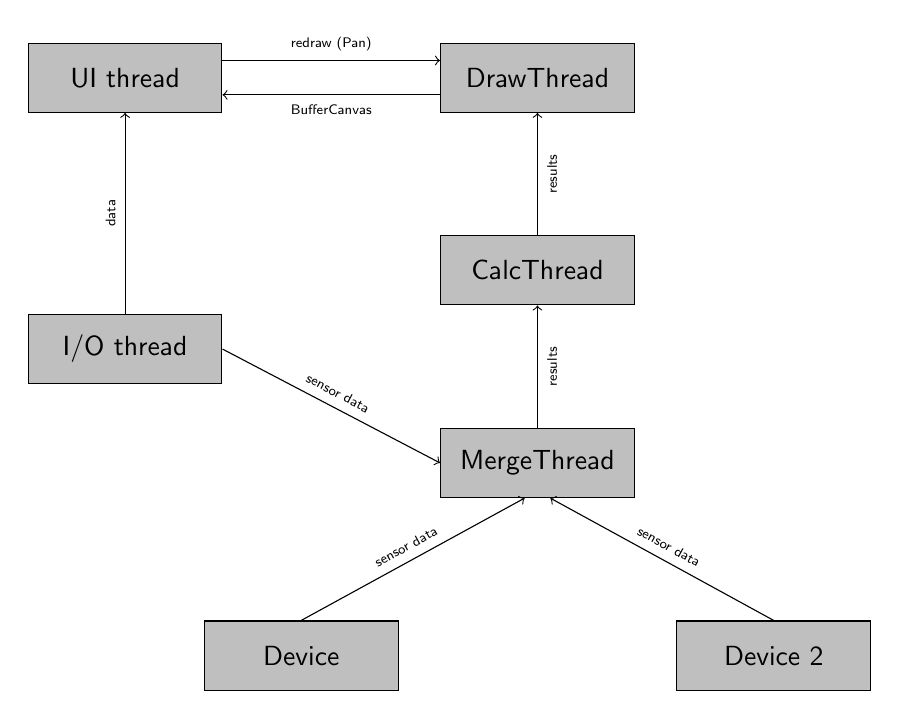
\begin{tikzpicture}
  \node(ui)[thread]{UI thread};

  \path(ui.east)+(4,0) node(draw)[thread]{DrawThread};
  \draw[->] (ui.10) -- (draw.170)
  node[midway, above, sloped, font=\tiny]{redraw (Pan)};
  \draw[->] (draw.190) -- (ui.350)
  node[midway, below, sloped, font=\tiny]{BufferCanvas};

  \path(draw.south)+(0,-2) node(calc)[thread]{CalcThread};
  \draw[->] (calc.north) -- (draw.south)
  node[midway, below, sloped, font=\tiny]{results};

  \path(calc.south)+(0,-2) node(merge)[thread]{MergeThread};
  \draw[->] (merge.north) -- (calc.south)
  node[midway, below, sloped, font=\tiny]{results};

  \path(merge.south)+(-3,-2) node(device1)[thread]{Device};
  \draw[->] (device1.north) -- (merge.250)
  node[midway, above, sloped, font=\tiny]{sensor data};

  \path(merge.south)+(3,-2) node(device2)[thread]{Device 2};
  \draw[->] (device2.north) -- (merge.290)
  node[midway, above, sloped, font=\tiny]{sensor data};

  \path(ui.south)+(0,-3) node(io)[thread]{I/O thread};
  \draw[->] (io.north) -- (ui.south)
  node[midway, above, sloped, font=\tiny]{data};
  \draw[->] (io.east) -- (merge.west)
  node[midway, above, sloped, font=\tiny]{sensor data};
\end{tikzpicture}

The UI thread is the main thread.  It starts the other threads and is
responsible for the UI event loop.  No other thread is allowed to
manipulate windows.  The UI thread has a timer which does regular
house keeping twice per second (\texttt{Pro\-cess\-Ti\-mer.cpp}).

The calculation thread (\texttt{Calcu\-la\-tion\-Thread.cpp},
\texttt{Glide\-Com\-pu\-ter*.cpp}) does all the expensive calculations
in background.  It gets data from the devices (through
\texttt{Merge\-Thread}) and forwards it together with calculation
results to the drawing thread and the main thread.

Each device has its own thread (\texttt{Serial\-Port.cpp}).  This is
needed because Windows CE does not support asynchronous COMM port I/O.
The thread is stopped during task declaration (which happens in the UI
thread).

When new data arrives on the serial port, the \texttt{Merge\-Thread}
gets notified, which will merge all sensor values into one data
structure.  It will then run cheap calculations, and forwards
everything to the \texttt{Calcu\-la\-tion\-Thread}.

With OpenGL, the map is rendered live without a buffer.  There is no
DrawThread.

On Android, the UI thread is not the main thread - the main thread is
implemented in Java, managed by Android itself.  The UI thread listens
for events which the Java part drops into the event queue
(\texttt{NativeView.java} and others).  The internal GPS does not need
a thread, it is implemented with Java callbacks.  For Bluetooth I/O,
there are two threads implemented in Java (\texttt{InputThread.java}
and \texttt{OutputThread.java}, managed by
\texttt{BluetoothHelper.java}).

\subsection{Locking}

Some data structures are rarely modified.  There is no lock for them.
For a modifications, all threads must be suspended.  Example:
waypoints, airspaces.

Other data structures are modified so often that correct locking would
be too much overhead.  Each thread and each instance has its own
copy.  The lock needs to be obtained only for making the private
copy.  The private copy can be used without locking.  Example:
\texttt{NMEA\_INFO}, \texttt{DERIVED\_INFO}.

There are objects which are too expensive to copy.  Normal locking
applies to them.  We have a template class called \texttt{Guard} to
enforce proper read/write locking.  Example: the task.


\section{Accessing Sensor Data}

Much of XCSoar deals with obtaining sensor data and visualising it.

Suppose you want to write a dialog that needs the current GPS
location, where do you get it?  The short and simple answer is: from
\verb|CommonInterface::Basic()| (the \texttt{InterfaceBlackboard}).
Example:

\begin{verbatim}
#include "Interface.hpp"

...
  const auto &basic = CommonInterface::Basic();
  if (basic.location_available)
    current_location = basic.location;
\end{verbatim}

This is true for the main thread (aka the ``user interface thread'').
Other threads must not use the \texttt{Interface.hpp} library, because
the \verb|InterfaceBlackboard| is not protected in any way.  It
contains copies of various data structures just for the main thread.

This is how sensor data moves inside XCSoar:

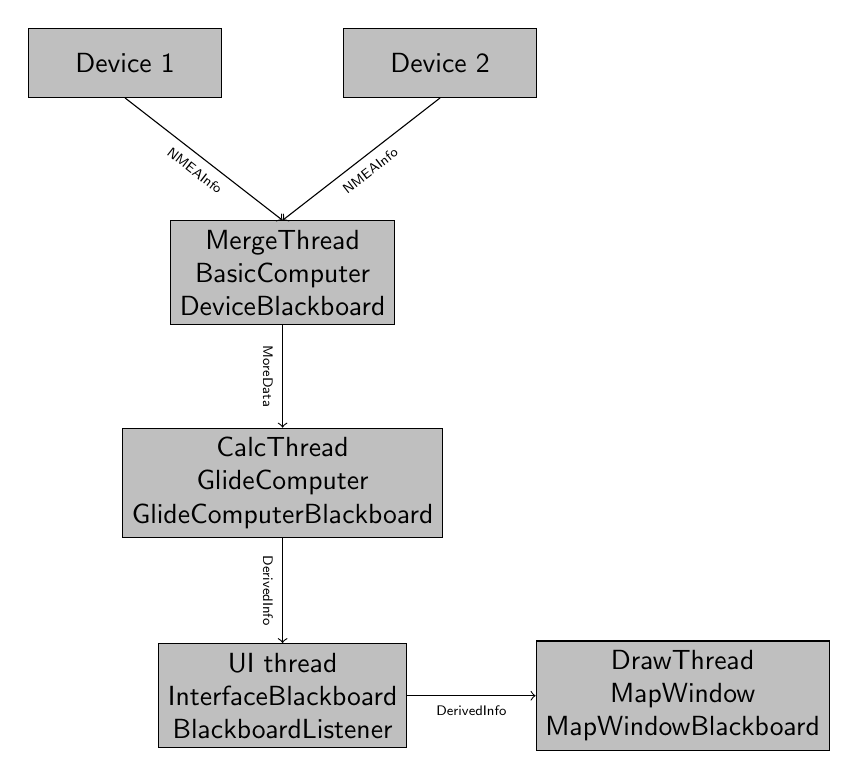
\begin{tikzpicture}
  \node(merge)[thread,align=center]{
    MergeThread\\
    BasicComputer\\
    DeviceBlackboard
  };

  \path(merge.north)+(-2,2) node(device1)[thread]{Device 1};
  \draw[->] (device1.south) -- (merge.north)
  node[midway, below, sloped, font=\tiny]{NMEAInfo};

  \path(merge.north)+(2,2) node(device2)[thread]{Device 2};
  \draw[->] (device2.south) -- (merge.north)
  node[midway, below, sloped, font=\tiny]{NMEAInfo};

  \path(merge.south)+(0,-2) node(calc)[thread,align=center]{
    CalcThread\\
    GlideComputer\\
    GlideComputerBlackboard
  };
  \draw[->] (merge.south) -- (calc.north)
  node[midway, below, sloped, font=\tiny]{MoreData};

  \path(calc.south)+(0,-2) node(ui)[thread,align=center]{
    UI thread\\
    InterfaceBlackboard\\
    BlackboardListener
  };
  \draw[->] (calc.south) -- (ui.north)
  node[midway, below, sloped, font=\tiny]{DerivedInfo};

  \path(ui.east)+(3.5,0) node(draw)[thread,align=center]{
    DrawThread\\
    MapWindow\\
    MapWindowBlackboard
  };
  \draw[->] (ui.east) -- (draw.west)
  node[midway, below, sloped, font=\tiny]{DerivedInfo};
\end{tikzpicture}

The device driver parses input received from its device into its own
\texttt{NMEAInfo} instance inside \texttt{DeviceBlackboard}
(i.e. \verb|per_device_data|).  Then it wakes up the
\texttt{MergeThread} to merge the new data into the central
\texttt{NMEAInfo} instance.  The \texttt{MergeThread} hosts the
\texttt{BasicComputer} which attempts to calculate missing data (for
example, derives vario from GPS altitude).

The \texttt{CalculationThread} wakes up and receives the
\texttt{MoreData} object from \texttt{DeviceBlackboard}.  Here,
expensive calculations are performed (\texttt{GlideComputer}: task
engine, airspace warnings, ...), resulting in a \texttt{DerivedInfo}
object.  The \texttt{CalculationThread} runs no more than twice per
second.

Finally, the UI thread wakes up and receives \texttt{MoreData} and
\texttt{DerivedInfo} via \texttt{DeviceBlackboard}.  This updates
InfoBoxes and other UI elements.  On Windows, the map is drawn in a
separate thread, so there's another layer.

Let's get back to the question: where do I get sensor data?  That
depends on who you are:

\begin{itemize}

\item you are the user interface: (InfoBoxes, dialogs, any Window
  callback): \texttt{InterfaceBlackboard} (see above).  To get
  notified on changes, register a \texttt{BlackboardListener} (and
  don't forget to unregister it).

\item you are the MapWindow: depends!  If you're being called from
  \texttt{OnPaintBuffer} (i.e.\ inside the \texttt{DrawThread}), you
  must use the \texttt{MapWindowBlackboard}, all others must use the
  \texttt{InterfaceBlackboard}.

\item you are a ``computer'' library: you will get the values as a
  parameter.  Don't try to use the \texttt{GlideComputerBlackboard}
  directly.

\item you are a device driver: implement the method
  \texttt{OnSensorUpdate} or \texttt{OnCalculatedUpdate} if you need
  to know values from other devices or calculation results.

\item everybody else may use the \texttt{DeviceBlackboard}, but be
  sure to lock it while using its data.

\end{itemize}


\chapter{Developing}

\section{Debugging XCSoar}

The XCSoar source repository contains a module for the GNU debugger
(\texttt{gdb}).  It contains pretty-printers for various XCSoar types,
including \texttt{Angle}, \texttt{GeoPoint} and others.  These are
helpful when you print values in the debugger.  To use it, start the
debugging session and load the module:

\begin{verbatim}
$ gdb -ex "source tools/gdb.py" output/UNIX/bin/xcsoar
(gdb) run
\end{verbatim}

The module will automatically convert fixed-point to floating point,
radian angles to degrees and more.  You can now do fancy stuff like:

\begin{verbatim}
(gdb) p basic.location
$1 = GeoPoint(7.93911242887 51.1470221074)
(gdb) p basic.date_time_utc
$2 = DateTime(2012/12/23 21:41:57)
(gdb) p basic.track
$3 = 55.2254197961
(gdb) p basic.external_wind
$4 = GeoVector::ZERO
(gdb) p current_leg.vector_remaining
$5 = GeoVector(267.899420345 107957.109724)
\end{verbatim}



%%%%%%%%%%%%%%%%%%%%%%%%%%%%%%%%%%%%%%%%%%%%%%%%%%%%%%%%%%%%%%%
\chapter{User interface guidelines}

\section{General}

\begin{itemize}
\item Minimise the number of colours, and re-use colour groups already defined.
\item Too much use of colour where it is not required serves only to reduce 
 the effectiveness of bright colours for important items.
\item High colour saturation elements should be reserved for high importance items
\item High contrast against background should be reserved for high importance items
\item Attempt to adopt colours that are intuitive based the function of the item
\item Minimise the clutter where possible --- readibility is essential for use 
 in flight
\item Use colours defined in \verb|Graphics| according to functional name, not 
 their actual colour.
\item Try to maintain consistent use of colours in all uses of that function, 
 such as dialogue graphics as well as map overlays and infoboxes.
\item Text should always be monochrome.
\end{itemize}

Use aviation conventions or adopt best aviation human factors
standards where possible, in particular:
\begin{itemize}
\item ICAO Internation Standards and Recommended Practices, Annex 4 to the 
 Convention on International Civil Aviation (Aeronautical Charts).
\item NASA Colour Usage recommendations and design guidelines: \verb|http://colorusage.arc.nasa.gov/|
\item DOT/FAA/AR-03/67 {\em Human Factors Considerations in the Design and 
 Evaluation of Electronic Flight Bags (EFBs)} \verb|http://www.volpe.dot.gov/hf/aviation/efb/docs/efb_version2.pdf|
\item FAA Human Factors Design Standards \verb|http://hf.tc.faa.gov/hfds/|.
\item DOT/FAA/AM-01/17 {\em Human Factors Design Guidelines for Multifunction Displays}
\end{itemize}

Check for performance with respect to colour blindness.
This site has a useful tool that can be used to convert screenshots
to how they would look to a person with common color blindness:
\verb|http://www.etre.com/tools/colourcheck/|.

{\bf For safety purposes, avoid use of elements that may encourage or require 
the user to stare at the screen continuously.}

{\bf For safety purposes, avoid user controls that have significant risk of 
producing unsafe results if misconfigured by the pilot.}

\subsection{General colour conventions}
Colour conventions generally in use throughout the program:
\begin{itemize}
\item Red for indicator of warning
\item Orange for indicator of caution
\item Green for positive indicator of safety
\item Blue for neutral indicator of safety
\end{itemize}

\subsection{Displayed data}
\begin{itemize}
\item Where data is invalid, indicate this by not presenting the data or
  showing dashes.
\item Present data in user-defined units.
\item Display numerical data with significant digits appropriate to the accuracy of the
  calculations, or its functional use by the pilot, whichever is lower.
\end{itemize}

\section{Dialogs and menu buttons}

\subsection{Colors}
Colour conventions in use are:
\begin{itemize}
\item Grey for buttons
\item Buttons and other widgets rendered with an evenly shaded border
\item Yellow for clicked items
\item Light blue for the key focused item
\item Medium blue for dialogue title bar
\item Text is black if the item is enabled
\item Text is greyed out (but still visible) if the item is disabled
\end{itemize}

\subsection{dialogue types and navigation buttons}
There are four types of dialogs in XCSoar, and the navigation 
buttons for each are different.  
Navigation buttons are the Close, OK, Cancel and Select buttons.
\begin{itemize}
\item Dialogs that modify and save data when the dialogue closes.

These shall usually have a Close button (no Cancel) and may have context specific 
function buttons
\item Dialogs that modify data where Cancel would be important for the user.

These shall have OK and Cancel buttons.  This may include dialogs with 
children dialogs where hitting Cancel from the parent dialogue cancels 
all the changes made in the children dialogs

\item Dialogs that have a list of values, one of which can be selected to 
 return to the parent dialogue.

These shall have Select and Cancel buttons
\item Dialogs that display information that cannot be modified.

These shall have a Close button
\end{itemize}

\subsection{dialogue button placement and size}
\begin{itemize}
\item The Close and Cancel buttons will never appear in the same dialogue and 
 are always located in the same place.  This location will be:

For portrait: lower right

For landscape: lower left
\item The Select button will be accompanied with a Cancel button.  The locations will be:

For portrait: Select in lower left, Cancel in lower right

For landscape: Cancel in lower left, Select immediately above it
\item Buttons will be 35 (scaled) pixels high
\item Buttons will be flush with the bottom of the screen and with the sides of 
 the screen and against each other (no margins)
\item In portrait, buttons will be 33% or 50% or 100% width of the screen
\item In landscape, buttons will be 65 to 80 (scaled) pixels wide, as wide as the 
 frame permits.  They will generally be a vertical row of buttons flush left of the screen
\item If text won't fit on a button, the buttons can be made larger consistently 
 for a screen, but this should be the exception because if it must contain that 
 much text consider using a different type of control.
\item Exceptions to all the dialogue concepts above are encouraged, but should be 
 mocked up and reviewed with the development community prior to implementing and 
 possibly documenting in the developers guide.
\end{itemize}

\subsection{Usability}
\begin{itemize}
\item Minimum size of buttons should be X by Y mm
\item Ensure all dialogs are navigable using cursor keys only
\item Ensure the focussed item is clearly identified.  The rectangle
  of the widget on the canvas may be drawn using the \verb|fill_focus| method
  of \verb|Canvas|.
\end{itemize}

\section{Main graphics}

\subsection{Colors}
Colour conventions in use, in order of priority, are:
\begin{itemize}
\item Aircraft black and white, for neutrality but clear identification
\item Traffic (FLARM) use alarm green, orange, and red.
\item Lift is vibrant green, sink is copper orange.
\item Aircraft navigation (route, best cruise track) is (ICAO) dark purple-blue
\item Task navigation lines and areas are (ICAO) magenta.
\item Updraft sources and other updraft derived data is sky blue.
\end{itemize}

(Todo) airspace alert colours

Map culture (topography) and terrain rendering should conform to ICAO
Annex 4 where appropriate.  Note that some modifications are
reasonable for electronic use given that Annex 4 deals with paper
charts.  Nevertheless, the colour conventions are useful to adopt as they are
likely to be intuitive and are designed for aviation use.

\subsection{Pen styles}

\begin{itemize}
\item Map culture should be rendered with a thin pen
\item Thicker pens used for important (e.g.\ task, navigational, airspace) lines
\item Dashed lines are used to increase perceptual priority
\end{itemize}

\subsection{Map overlays}
Elements on the map that are not part of the map layer, such as additional
informational widgets (final glide bar, wind, north arrow) should be rendered
so as to help those elements be visually separated from the map:

\begin{itemize}
\item Generally adopt higher contrast (higher colour saturation or darker shade) 
 than the background map layer elements.

\item For elements covering an area (non line), draw the entire element or a border
with a luminosity contrasting pen, of width \verb|IBLSCALE(1)|.

\item Consider whether the widget is required in all flying states and display modes.
if it does not serve a direct functional purpose in some states/modes, do not
render it.

\item Avoid locating widgets at the aircraft symbol (ownship symbol).
It is important to keep this area clear so the aircraft symbol can be easily found.

\end{itemize}

Elements that may be rendered over each other should be organised in order of
priority, particularly with alert warning items above caution items above non-alert items.

\section{Terminology}
\subsection{Glide Ratio}
'Glide ratio' is a non-specific term which can refer to the ratio of horizontal to 
vertical motion with reference to either the surrounding airmass or the ground.

To reduce confusion, ground-referenced glide ratios (eg distance travelled over 
ground vs altitude lost) should be referred to by the term 'glide ratio over 
ground' when space allows, or 'glide ratio' / 'GR'.

Air-referenced glide ratios (eg airspeed vs sink rate) should be specified as 
'lift/drag ratio' / 'L/D ratio' / 'LD'. The lift/drag ratio is numerically equal 
to the air-referenced glide ratio when flying at constant speed.

If usage spans both air-referenced and ground-referenced glide ratios, the 
non-specific term 'glide ratio' / 'GR' should be used. 'Lift/drag ratio' should 
never be used to refer to ground-referenced glide ratios.

\chapter{File formats}\label{cha:file_formats}

\section{Input Events}

\warning The Input System is deprecated!  It is being replaced by a
Lua scripting engine.

\subsection{Introduction}

The Input System is actually a large number of things all bunched into one.

Primarily it is about giving the user control of what button does what
and when. There is a new concept called Input Mode - this is a the
mode the GUI is in for input. For example, you can click on the info
boxes and you are now in "infobox" mode. Clicking on the map is called
"default". But it doesn't stop there, you can create a new mode called
anything you like. This may not mean much - but wait till you combine
it with the rest of the features...

Input is not restricted to hardware buttons any more. You can map all
your hardware buttons (currently support for APP1 to APP6, Left,
Right, Up, Down and Enter, although I believe we can do some more) but
also any key code at all. This feature allows those with a built in
keyboard to use any key to map to any function in XCS. Where it comes
into real advantage is in external keyboards. There are a number of
bluetooth devices out there (eg: \url{http://shop.brando.com.hk/btgamepad.php}) 
which can map each of their
buttons to any key code - that key code can then be mapped to any
feature in XCS. You can then add to the hardware buttons the buttons
available to you on external devices. Other inputs (eg: Serial) are
also being looked at - and support is in the code for that extension.

We are striving towards a platform which is not only easier to use and
more intuitive, but also faster and easier to use in flight as
well. As such, another new feature as part of input is the concept of
Button Labels. Combined with the modes mentioned above, you can create
any arbitrary set of functions to map to any number of buttons. Think
about it like creating a tree, or a multiple level menu.

This produces two benefits that I know will be appreciated by people
with limited inputs. The first is that you can create menus, where by
you press one button to get to the next level (eg: pressing on APP1
brings up AutoZoom, Pan Mode, Full screen on the other buttons. Press
APP1 again and it goes to Terrain, Marker and Auto MacCready. Press
APP1 again and the menu is gone) - but more importantly for those with
touch screens and limited buttons, each of these labels can optionally
be assigned a key and you can touch the button area as if it was a
button.  This means that we can actually control on a touch screen
model the entire system without buttons - press an area of the screen
and the buttons pop up, click through - change options and more.

The combined features of labels, configurable buttons (including from
external hardware), hierarchical menus (for lack of a better name),
touch screen buttons has allowed us to configure XCS - without
recompile - for an enormous range of hardware, and personal
preference.  And all configurable as plane text, simple files. There
is no need for a file, the defaults internally will probably be a
combination of a 4 button bottom system with one button always shown
on screen for no/few button display.

The screen layout - location of the labels - is also totally
configurable - allowing us to vary the layout of buttons depending on
the type of organiser or desired look and feel.

There is a great unexpected benefit in the development of the input
system.

We can execute any number of events attached to an input with only 2
extra lines of code. This worked perfectly. So now we have a basic
macro system, allowing many more events to be attached to a single
input event.

But it doesn't stop there, this has lead to some more excellent
developments. The idea of Glide Computer Events things like "Maximum
Altitude Reached". Currently we play a sound effect for that. But you
may choose to play a sound, bring up a message box and write to the
log file.

One nice feature of XCS is the ability to change things such as Zoom
and North when Circling. Now you can do so much more. You could choose
to point North, Zoom to 1.0 (rather than a relative change), Turn on
Vario Sounds, Start a timer. When switching back to Cruise mode, you
can bring up the stats box for 30 seconds. The options are limited by
your imagination.

This is also contributing to a major reduction in complex code. We can
move out these complex tests into one centrally, easier to manage
system, reducing bugs and improving maintainability.

Another side benefits of these Macros is User Defined Flight
Modes. One idea was a button which switched to Zoom 1.0, Pan ON, Pan
Move to Next Waypoint. Basically the ability to jump and see the next
waypoint. And in the previous we can change the Input Mode to
"ViewWaypoint" - at which point you can redefine the same button to
switch back to your original settings.

The flexibility of this system comes with only one small price. We
can't provide an interface within XCS to fully customise all of these
near infinitely variable possibilities. However I believe that is
unnecessary anyway, you are not likely to change these sort of
features very often, and definitely not on the field. That does not
mean you can't, you can of course edit the plane(sic) text file to
change functions.

What this really means is that we can have people in the project
helping and contributing to the customising of XCS, without having to
change the code. This, especially on an open source project is
fantastic as it nicely separates the user interface changes from the
highly reliable part of the code. It also involves people who can
develop new interfaces and functions that are expert gliders but not
necessarily programmers.

For information on file formats see Common/Data/Input/template.xci and
the web site documentation.


\subsection{Defaults and Files}

The file in the source Common/Data/input/template.xci is used to generate
automatically the C code necessary for the default configuration. However it is
in the exact same format as can be read in by XCS and therefore can be used
literally as a template for a more complicated file.

When you create your own file, you will need to select it as the Input File
within XCSoar Menu/Settings/Input Files, and then restart XCS.


\subsection{File format}

The file is plain text, with key=value pairs and a blank line to indicate
the end of a record.

\begin{verbatim}
mode=default
type=key
data=APP1
event=StatusMessage My favorite settings are done
event=ScreenModes full
event=Sounds on
event=Zoom 1.0
event=Pan off
label=My Prefs
location=1
\end{verbatim}

The record above demonstrates remapping the first hardware key on your
organiser to change Pan to off, Zoom to 1.0 Sounds on, ScreenModes
full, and then a status message to tell you it is done.

Lines are terminated by the stanard DOS newline which is CRLF (Carrage
Return then Line Feed). Records are terminated by an extra new line.

\subsection{Event order}

Until further work is done on processing, events are actually done in
reverse order - also known as RPN. This is because the events work on
the stack principle. Each one is pushed onto the stack for execution,
and then executed by popping back off the stack. This has reduced
complexity of the code base.

When writing input events, have a look where you put the StatusMessage
and make sure that it is at the top, not the bottom (if you have one).

\subsection{Event list}

{\footnotesize
\begin{tabular}{l|p{7cm}}
\emph{Event} & \emph{Description} \\

\hline

\texttt{MainMenu} & \\

\hline

\texttt{MarkLocation} & Mark a location. \\

\hline

\texttt{Mode} \emph{M} & Set the screen mode. \\

\hline

\texttt{Pan} \emph{P} & Control pan mode.  Possible arguments: on
(enable pan), off (disable pan), up, down, left, right \\

\hline

\texttt{PlaySound} \emph{S} & Play the specified sound. \\

\hline

\texttt{SnailTrail} \emph{S} & Change snail trail setting.  Possible
arguments: off, short, long, show. \\

\hline

\texttt{ScreenModes} \emph{M} & Set the screen mode.  Possible
arguments: normal, auxilary, toggleauxiliary, full, togglefull,
toggle. \\

\hline

\texttt{Sounds} \emph{S} & Change vario sounds.  Possible arguments:
toggle, on, off, show. \\

\hline

\texttt{StatusMessage} \emph{M} & Display the specified status
message. \\

\hline

\texttt{Zoom} \emph{Z} & Everything about zoom of map.  Possible
arguments: auto toogle, auto on, auto off, auto show, in, out, +, ++,
-, --. \\

\end{tabular}}

\subsection{Modes}

XCSoar now has the concept of Modes. These are an arbitrary
string that associates with where and what XCS is doing.

Note: a mode entry in a record can have multiple entries by using a space
between eg: "infobox menu1 menu2"

\subsubsection{List of known modes}

\begin{description}
\item[\texttt{default}] Really map mode, where you mostly are
\item[\texttt{infobox}] An info box has been selected on the scrreen
\item[\texttt{*}] Any other arbitrary string
\end{description}

Mode precedence has been tricky, so instead of solving the problem 
it is being worked around. XCS will choose to set a global variable 
to specify what mode it thinks it is in. This can then be used by the
input code to decide what to do. This mode could get out of sink
with the real world, and careful checking will be required, but at
this stage it seems like the only sensible option.

The code will review first if an entry exists in the current mode, and 
then in the default mode. This allows you to do one of the following
example: Define a default action for button "A" to be "Zoom In" but
make that button increase Bugs value in infobox mode only. You can do
this by making an "default" and a "infobox" entry. You can also put an entry
in for Button "A" for every mode and have complete control.

Special Modes - eg: the level of a menu (Think File vs Edit, vs Tools vs Help)

have special modes, such as
the level of the menu you are at. You press one button, then another
set become available (like pressing menu and seeing Settings etc). This
will be very useful in non-touch screen models. The menu configuration
can then be read from this same file and configured, allowing any
number of levels and any number of combinations.

The only hard part is what mode to go back to. We need a 
"Calculate Live Mode" function - which can be called to calculate the
real live mode (eg: finalglide vs curse) rather than the temporary
mode such as Menu, Special Menu Level, Warning etc.

The label and location values are examples of what can be done here
to allow input button labels to be displayed. What needs to be 
considered is a simple way of mapping the locations and the size.
In some models it may be that buttons are 4 across the top of the
screen, where as others it is 3 or 2 or even 6. So both size and
location needs to be considered.

The label itself will go through gettext to allow language
translations.

\subsection{Keys}

The key type can have the following possible values:

\begin{description}
\item[\texttt{APP1-APP6}] Hardware key on pocket pc
\item[\texttt{F1-F12}] Standard function keys
\item[\texttt{LEFT, RIGHT, UP, DOWN, RETURN}] Mapped to arrow keys - joystick on
  organisers
\item[\texttt{A-Z, 0-9}] and other possible keyboard buttons (case is ignored)
\end{description}


XXX Review...
Input Types

Types:

hardware	These are the standard hardware buttons 
on normal organisers. Usually these are
APP1..6.

keyboard	Normal characters on the keyboard (a-z etc)

nmea		A sentence received via NMEA stream (either)

virtual		Virtual buttons are a new idea, allowing
multiple buttons to be created on screen.
These buttons can then be optionally mapped
to physical buttons or to a spot on the 
screen (probably transparent buttons over 
the map).

Modifiers

It is a long term goal of this project to allow modifiers for keys.
This could include one of the following possibilities:

\begin{itemize}
\item Combination presses (although not supported on many devices)
\item Double Click
\item Long Click
\end{itemize}

Modifiers such as the above will not be supported in the first release.

\begin{verb}
Functions/Events - what it does

AutoZoom		on, off, toggle 
FullScreen		on, off, toggle
SnailTrail 		on, off, long, toggle
VarioSound 		on, off
Marker 			optional text to add
MenuButton 		on, off, toggle
Menu			open, close, toggle
MenuEntry		task, b+b, abortresume, abore, resume, pressure
logger, settings, status, analysis, exit, cancel
NOTE: Some of the above may be separate functions
Settings		(each setting, bring up to that point)
Bugs			add, subtract, 0-100% (set value)
Ballast			add, subtract, 0-100% (set value)
Zoom			add, subtract, 0-nn (set value)
Wind			up, down, 0-nn (set value, left, right, "n","ne","e","se","s","sw","w","nw"...
MacCready		add, subtract, 0-nn (set value)
WaypointNext		"String" to specific waypoint
eg: WayPointNext "home"
WayPoint???		"reverse" - reverse, from last passed back to start (ie: from here to home)
"drop next" - drop the next
"restore" - restore all - from start of flight but 
XXX This needs more thought
flight 			"startstop", "start", "stop", "release"
Start/Stop of flight - Can be automatic, but pressing will override
automatic part.
release 		markse the point of release from tow
\end{verb}

\subsection{Glide Computer Events}

These are automatically triggered events. They work in exactly the
same way, but instead of the user pressing a key, the glide computer
triggers the events.

A simple example is moving from Cruise to Climb mode. We want to zoom
in, change our track up to north up and switch to full screen. You may
also choose to drop a marker with the words "entered thermal". The
choicese are up to your imaginations - the GCE (Glide Computer Events)
allow you to control what happens.

These are represented as "type=gce" and data=* - as listed below.

{\footnotesize
\begin{tabular}{l|p{5.6cm}}
\emph{Event} & \emph{Description} \\
\hline

\verb|COMMPORT_RESTART| & The comm port is restarted. \\

\hline

\verb|FLIGHTMODE_CLIMB| & The flight mode has switched to ``climb''. \\

\hline

\verb|FLIGHTMODE_CRUIS| & The flight mode has switched to ``cruise''. \\

\hline

\verb|FLIGHTMODE_FINALGLIDE| & The flight mode has switched to ``final
glide''. \\

\hline

\verb|GPS_CONNECTION_WAIT| & Waiting for the GPS connection. \\

\hline

\verb|GPS_FIX_WAIT| & Waiting for a valid GPS fix. \\

\hline

\verb|HEIGHT_MAX| & Maximum height reached for this trip. \\

\hline

\verb|LANDING| & You are at landing. \\

\hline

\verb|STARTUP_REAL| & First message - this happens at startup of the
real XCS. \\

\hline

\verb|STARTUP_SIMULATOR| & Startup first message. This happens during
simulator mode. \\

\hline

\verb|TAKEOFF| & You have taken off. \\

\end{tabular}}

\section{Map Data file formats}
The map data is typically downloaded from the map generator server and consists of a single \texttt{.xcm} file.
It is a zip file which contains several separate files for terrain, topography and waypoint data:
\begin{itemize}
\item[\texttt{info.txt}] General map information
\item[\texttt{terrain.jp2}] Terrain (elevation) data, georeferenced in \texttt{terrain.j2w}
\item[\texttt{waypoints.cup}] Waypoint data
\item[\texttt{topology.tpl}] Topography data file index
\item[\texttt{*.shp} / \texttt{*.dbf} / \texttt{*.shx}] A set of ESRI format shape file sets with actual topography voctor data information, as listed and defined in \texttt{topology.tpl} (Coasts, rivers, roads, cities etc.)
\end{itemize}
\subsection{Map information}
\texttt{info.txt}
Contains information about the map as a whole, such as creator, creation time, and lat/lon range.

\subsection{Terrain data files}
The map cointains a digital elevation model of the map area. It is stored as an JPEG2000 compressed image in the file \texttt{terrain.jp2}. The projection information (lat/lon boundaries) of the DEM file are contained in the text file \texttt{terrain.j2w}, in decimal degree latitude/longitude format.
Water is defined as elevation lower than \texttt{TERRAIN\_WATER\_THRESHOLD=-30000}, therefore care has to be taken that JPEG compression parameters and algorithms  are used which do not generate artefacts at the coastlines due to the potentially big jump in elevation value.
\subsection{Waypoints}
A map database file can contain waypoints. They reside in the \texttt{waypoints.cup} file, which has regular \texttt{.CUP} format.

\subsection{Topography data}
\subsubsection{Shape files}
Non-elevation topography data is stored in standard ESRI shape files. For each type of topographic shape (road, river, city outline, etc.) there is one shape filein \texttt{.shp}, which containes all shapes of this type. For each \texttt{.shp} file, there has to be an associated \texttt{.dbf} file containing shape metadata (such as the name of the city) in dBASE format, and an index file of \texttt{.shx} file type which contains the index that relates the metadata to the shapes. 

All of this is defined in the ESRI shape file standard. The official definition of the standard can be found at\\ \href{http://www.esri.com/library/whitepapers/pdfs/shapefile.pdf}{http://www.esri.com/library/whitepapers/pdfs/shapefile.pdf}, but there are more compact descriptions available on the web, see for example wikipedia info and links at \\ \href{http://en.wikipedia.org/wiki/Shapefile}{http://en.wikipedia.org/wiki/Shapefile}.

There can be more files associated with each shape file, such as \texttt{.prj}, \texttt{.qix}, \texttt{.atx}, which are not used by XCSoar.

The set of shapefiles actually used by XCSoar and the attributes of each file are defined in the topography layer description file \texttt{topology.tpl}. All shape files used by the map must be listed there.

\subsubsection{Topography layer description file (topology.tpl) format}

Each line of the topography layer description file (\texttt{topology.tpl}) contains
a comma separated list (CSV) of information needed for rendering of an
individual topography layer. Lines starting with '*' are ignored.

XCSoar v6.6 and earlier will display at most 20 topography layers.
XCSoar v6.7 and later will display at most 30 topography layers.
\begin{table}[ht]
\centering
\sffamily
\begin{tabular}{@{}lll@{}}
\toprule
\addlinespace
Column name&Data type&Valid range\\
%\midrule
\cmidrule(r){1-1}\cmidrule(lr){2-2}\cmidrule(l){3-3}
filename&string&\\
range&double (nm)&-\\
icon&string&\\
label index&int&0-1\\
color (red component)&int&0-255\\
color (green component)&int&0-255\\
color (blue component)&int&0-255\\
pen width&int&0-31\\
label range (nm)&double&-\\
important label range (nm)&double&-\\
alpha&int&0-255\\
%\addlinespace
\bottomrule
\end{tabular}
\caption{Topography file format}
\label{tab:topography-file-format}
\end{table}

\begin{description}
\item[filename] The filename of the Topography layer within the container file.
\item[icon] XCSoar v6.5 and earlier, Only the value 219 is recognised, for town icons.
From XCSoar v6.6, the name of the icon to display. Optional. See below for a list of available names.
\item[range] Zoom level threshold. Layer elements will not be drawn unless zoomed in closer than this threshold.
\item[pen width] Lines contained within this layer are drawn with pen width.
\item[label range] Label display zoom level threshold. Labels contained in the layer file
will not be rendered unless zoomed in closer than this threshold.
\item[important label range] A zoom level threshold. Labels contained in the layer file will be
rendered in standard style when the display zoom level is greater than this threshold.
\item[alpha] The alpha component controls transparency of polygons...
0 means polygons are completely transparent, 255 means they are completely opaque.
Only used by XCSoar v6.7 and later.

\texttt{Versions of XCSoar running on Windows and WinCE ignore any item where transparency is specified.}

\end{description}
\subsubsection{Point Features}
Prior to XCSoar v6.6, this could contain the value 219 to display an icon for a town
From XCSoar v6.6, a user can put an optional string into the icon column in topology.tpl in the .XCM file (e.g.)
\begin{itemize}
\item SpotHeight,5,\texttt{mountain\_top},1,64,64,64,1,5,
\item Mast,10,\texttt{obstacle},,,,,1,10,
\end{itemize}
This can be used for Shapefiles containing point features or polygons or linestrings, but is probably only useful for point features.

The icon of the corresponding image and optional label will be displayed. In the first example, 
the "mountain\_top" icon and a label will be displayed for each point in the SpotHeight shapefile. My
SpotHeight Shapefile has been generated with the point elevation in feet as the label value). For the second example, only "obstacle" icons 
(no labels) will be displayed for points in the Mast Shapefile..

Icon names are detected in TopographyStore.cpp. Names must be given in lowercase. If the icon name given is unknown, or no icon name is given, then icons are not displayed for that Shapefile.


Names correspond to images which have been linked into XCSoar, although
it is envisaged that in future these will be names of icon files. Available icon names are:
\begin{itemize}
\item mountain\_top 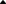
\includegraphics[angle=0,width=8pt,keepaspectratio='true']{icons/map_mountain_top.pdf}
\item bridge 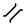
\includegraphics[angle=0,width=8pt,keepaspectratio='true']{icons/map_bridge.pdf}
\item tunnel 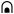
\includegraphics[angle=0,width=8pt,keepaspectratio='true']{icons/map_tunnel.pdf}
\item tower 
\includegraphics[angle=0,width=8pt,keepaspectratio='true']{icons/map_tower.pdf}
\item power\_plant 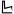
\includegraphics[angle=0,width=8pt,keepaspectratio='true']{icons/map_power_plant.pdf}
\item obstacle 
\includegraphics[angle=0,width=8pt,keepaspectratio='true']{icons/map_obstacle.pdf}
\item mountain\_pass 
\includegraphics[angle=0,width=8pt,keepaspectratio='true']{icons/map_pass.pdf}
\item weather\_station 
\includegraphics[angle=0,width=8pt,keepaspectratio='true']{icons/map_weather_station.pdf}
\item thermal\_hotspot
\item town
\item mark 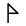
\includegraphics[angle=0,width=8pt,keepaspectratio='true']{icons/map_flag.pdf}
\item turnpoint 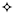
\includegraphics[angle=0,width=8pt,keepaspectratio='true']{icons/map_turnpoint.pdf}
\item small
\item cruise 
\includegraphics[angle=0,width=8pt,keepaspectratio='true']{icons/mode_cruise.pdf}
\item terrainwarning
\item logger
\item loggeroff
\item target
\item teammate\_pos
\item airspacei
\item traffic\_safe
\item traffic\_warning
\item traffic\_alarm
\item taskturnpoint
\item marginal 
\includegraphics[angle=0,width=8pt,keepaspectratio='true']{icons/winpilot_marginal.pdf}
\item landable 
\includegraphics[angle=0,width=8pt,keepaspectratio='true']{icons/winpilot_landable.pdf}
\item reachable 
\includegraphics[angle=0,width=8pt,keepaspectratio='true']{icons/winpilot_reachable.pdf}
\item airport\_reachable 
\includegraphics[angle=0,width=8pt,keepaspectratio='true']{icons/alt_reachable_airport.pdf}
\item airport\_unreachable 
\includegraphics[angle=0,width=8pt,keepaspectratio='true']{icons/alt_landable_airport.pdf}
\item airport\_marginal 
\includegraphics[angle=0,width=8pt,keepaspectratio='true']{icons/alt_marginal_airport.pdf}
\item airport\_unreachable2 
\includegraphics[angle=0,width=8pt,keepaspectratio='true']{icons/alt2_landable_airport.pdf}
\item airport\_marginal2 
\includegraphics[angle=0,width=8pt,keepaspectratio='true']{icons/alt2_marginal_airport.pdf}
\item outfield\_unreachable2 
\includegraphics[angle=0,width=8pt,keepaspectratio='true']{icons/alt2_landable_field.pdf}
\item outfield\_marginal2 
\includegraphics[angle=0,width=8pt,keepaspectratio='true']{icons/alt2_marginal_field.pdf}
\item outfield\_reachable 
\includegraphics[angle=0,width=8pt,keepaspectratio='true']{icons/alt_reachable_field.pdf}
\item outfield\_unreachable 
\includegraphics[angle=0,width=8pt,keepaspectratio='true']{icons/alt_landable_field.pdf}
\item outfield\_marginal 
\includegraphics[angle=0,width=8pt,keepaspectratio='true']{icons/alt_marginal_field.pdf}
\end{itemize}
\subsubsection{Adding new Icons}
At the moment, adding new icons requires a rebuild of the XCSoar application.It is envisaged that, in future, 
this process won't be required... users will include icon files in their .XCM map container files, and refer to them 
by name. However, that has not yet been implemented. 

To add your own images to the list of icons:
\begin{enumerate}
\item Create a .svg file for the icon (e.g. mast.svg) and copy into \texttt{xcsoar/Data/icons}. For Android, the name must be lowercase.
\item Insert two (for normal and high-res) lines into \texttt{xcsoar/Data/XCSoar.rc},  (e.g.)
\begin{verbatim}
BITMAP\_ICON(IDB\_MAST, "mast")
BITMAP\_ICON(IDB\_MAST\_HD, "mast\_160")
\end{verbatim}
\item Insert two lines into \texttt{xcsoar/src/Resources.hpp} (e.g.)
\begin{verbatim}
MAKE_RESOURCE(IDB_MAST, 500);
MAKE_RESOURCE(IDB_MAST_HD, 5500);
\end{verbatim}
\item Add a corresponding line into the \texttt{icon\_list} table in \texttt{xcsoar/src/Topography/TopographyStore.cpp}
\begin{verbatim}
  {"mast", IDB\_MAST},
\end{verbatim}
\item Make XCSoar
\end{enumerate} 
After this, a line can be added in \texttt{topology.tpl} to connect the icon to the Shapefile using the icon name. (e.g.)
\begin{verbatim}
Mast,10,mast,,,,,1,10,
\end{verbatim}

Note that unless these changes are merged into the main XCSoar repository, then only your specific build of XCSoar will be able to 
display your icon image.



%%%%%%%%%%%%%%%%%%%%%%%%%%%%%%%%%%%%%%%%%%%%%%%%%%%
\appendix

\chapter{Setting up a development environment based on linux}\label{cha:developmentsetup}
This describes the setup of a development environment suitable to compile \xc
for most supported platforms. The manual focuses on recent releases of
Debian-based flavors of GNU/Linux (including Ubuntu).

In the following instructions, \texttt{sudo} is used to execute commands with
root privileges. This is not enabled by default in Debian (but on some Debian
based distributions, like Ubuntu).

To install a virtual machine with the required, you can use \texttt{Vagrant},
see section \ref{sec:vagrant}.

\section{Download source code}
To download the \xc source code, make sure you have git installed:
\begin{verbatim}
sudo apt-get update
sudo apt-get install git
\end{verbatim}

Download the source code of \xc by executing \texttt{git} in the following way in
your project directory:
\begin{verbatim}
git clone git://github.com/XCSoar/XCSoar

# download submodule
cd xcsoar
git submodule init
git submodule update
\end{verbatim}

\section{Use provisioning scripts}
If you are not using Vagrant, but an existing standard installation of a
Debian-based Linux distribution, you can run the scripts from
\texttt{ide/provisioning} subfolder of the \xc source to install the build
dependencies for various \xc target platforms.

\begin{verbatim}
cd ide/provisioning
sudo ./install-debian-packages.sh
./install-android-tools.sh
\end{verbatim}

\section{Optional: Eclipse IDE}
One of the most widespread IDEs is eclipse. It is not limited to Android, and can be used for all targets. It is not required for \xc, but its installation is described here as an example. Eclipse is quite heavyweight, and many developers prefer other IDEs for \xc development.

To install, download the eclipse installer (Sometimes called "\emph{Ooomph!}" for some reason) from here:\\
\texttt{https://www.eclipse.org/downloads/}

Important: Install the CDT version of eclipse for C development, not the Android/Java package, even if you plan developing for Android. In addition, it is very convenient to install the git support (egit).

The current stable version is \emph{eclipse mars} (4.5) and works with OpenJDK 7 or 8, the new \emph{eclipse neon} 4.6, currently RC2, is also quite stable, and requires OpenJDK 8. Both can be installed with the installer.

You can also install the ADT (Android development tools) package for better integration with Android.

Next, create a new project, by generating a make project from existing sources files. Choose your xcsoar source directory which contains the makefile.

Important: After you have added the sources, eclipse will start indexing all files. If you have already started \texttt{make} before this time, then a lot of files have been downloaded for the various libraries which are exctracted/built within the \xc directory (most notably the boost libraries). Indexing all these takes a very long time, and a lot of heap space, so you should probably stop the indexer right away. In addition you should probably exclude these directories from the indexer for the future.

For this, in the C/C++ scope, right-click on the "output" directory in the file tree on the left side, select "Properties", then "Resource/Resource Filters" and add a filter. In the "add filter" dialog, choose "exclude all", "files and folders", "all children (recursive)" and set the Filter details to "Name matches *".
This will exclude the output tree from the indexer, leading to a minimal index.

\section{Optional: modern LaTeX editor for editing the Manual}
Most people today edit LaTeX files in specific editors, as this is much more comfortable and efficient. This is highly recommended especially if you are not very familiar with LaTeX: learning it is very easy with a modern editor. Here, we install TeXstudio as an example, as it is very widespread and supports the rather rare LuaLaTeX well.

To install, get the relevant package:

\begin{verbatim}
sudo apt-get install texstudio
\end{verbatim}

As the directory tree of \xc is very unusual for a LaTeX project, we need to make some special configurations in order to allow for quick compiling from within the editor, and for full synctex functionality:

In "Options / Configure TeXStudio", enable "show advanced options".

In "Options / Configure TeXStudio / Commands / Commands / LuaLaTeX", replace
\begin{verbatim}
lualatex -synctex=1 -interaction=nonstopmode %.tex
\end{verbatim}
with
\begin{verbatim}
lualatex -synctex=1 -interaction=nonstopmode
 -output-directory=?a)../../../output/manual %.tex
# Android SDK
export ANDROID_SDK_HOME="~/opt/android-sdk-linux_x86"
export PATH="$PATH:$ANDROID_SDK_HOME/tools"
export PATH="$PATH:$ANDROID_SDK_HOME/platform-tools"

# Android NDK
export ANDROID_NDK_HOME="~/opt/android-ndk-r16"
export PATH="$PATH:$ANDROID_NDK_HOME"
\end{verbatim}

In "Options / Configure TexStudio / Build / Build Options / Addition Search Paths":\\
Enter in \emph{both} fields ("Log file" and in the field "PDF File"):
\begin{verbatim}
../../../output/manual/
\end{verbatim}


Add the following line to \emph{both} the \texttt{.profile} and the \texttt{.bashrc} file of your user directory:
\begin{maxipage}
\begin{verbatim}
export TEXINPUTS="..:../../../output/manual:../../../output/manual/en:../../..:"
\end{verbatim}
\end{maxipage}


Finally, you need to run "make manual" in the \xc base directory at least once from the command line before you can compile from within the TexStudio interface. This creates the path structure and generates the figure files which are included into the manual. Of course, if you change figures, you might have to run "make manual" again.

Inside TeXStudio, open the file "XCSoar-manual.tex" (or one of the other root files) and right-click on this file to "set as explicit root document", in the structure view on the left. Now you are good to go. Make changes and press F5 to see the result immediately.


\chapter{GNU General Public License}\label{cha:gnu-general-public}
\input{gpl.tex}

\end{document}
